\chapter{Campos gauge, escalas de interacción y corrientes débiles cargadas}

La electrodinámica cuántica y la cromodinámica cuántica parecen muy distintas en el laboratorio, pero ambas son teorías gauge. De hecho, casi todas las interacciones del modelo estándar se organizan de este modo. La palabra \emph{gauge} tiene un significado más profundo relacionado con la simetría local, pero podemos dejar de lado por ahora ese formalismo. De momento necesitamos una descripción física mínima: una teoría gauge contiene campos de tipo Maxwell, fuentes conservadas, transformaciones de simetría, bosones gauge y reglas para emitir y absorber esos bosones.

\section{La teoría de Maxwell como prototipo}

\subsection{Campos y potenciales}

El campo electromagnético tiene seis componentes: tres del campo eléctrico y tres del campo magnético. La misma información puede codificarse, con cierta redundancia, en un potencial de cuatro componentes
\begin{equation}
A_\mu=(A_0,\boldsymbol A),
\end{equation}
donde \(A_0\) es el potencial electrostático y \(\boldsymbol A\) es el potencial vectorial espacial. En el límite electrostático, el campo eléctrico se obtiene a partir del gradiente espacial:
\begin{equation}
\boldsymbol E=-\boldsymbol\nabla A_0,
\qquad
\boldsymbol F=q\boldsymbol E,
\end{equation}
mientras que el campo magnético es
\begin{equation}
\boldsymbol B=\boldsymbol\nabla\times\boldsymbol A.
\end{equation}
El signo de la primera ecuación depende de la definición estándar del potencial; en la explicación en la pizarra interesa sobre todo que los campos son derivadas de los potenciales.
\editorialnote{Para campos dependientes del tiempo, la relación completa es
\(\boldsymbol E=-\boldsymbol\nabla A_0-\partial_t\boldsymbol A\). Aquí, la clase trabaja deliberadamente con el caso electrostático más sencillo.}

\begin{figure}[htbp]
\centering
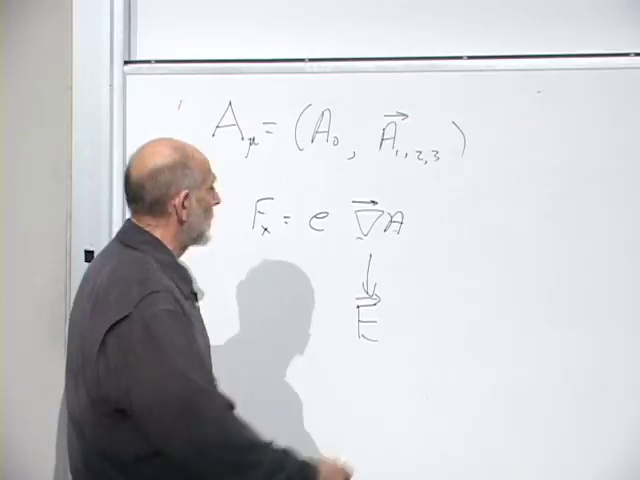
\includegraphics[width=0.62\textwidth]{lecture_05_figure_02.png}
\caption{El potencial electromagnético de cuatro componentes y su relación, mediante derivadas, con el campo.}
\lectureframe{00:03:33}
\end{figure}

Así pues, la electrodinámica admite dos descripciones equivalentes: una en términos de \(\boldsymbol E\) y \(\boldsymbol B\), y otra en términos de \(A_\mu\). Esta última solo tiene cuatro componentes explícitas porque distintos potenciales pueden describir los mismos campos físicos. Esa redundancia es el primer indicio del significado de la palabra gauge, aunque todavía no la usaremos de manera formal.

\subsection{Ondas y polarización}

Las ecuaciones de Maxwell admiten ondas. Consideremos una onda plana que se propaga en la dirección del vector unitario \(\hat{\boldsymbol k}\). En cada punto, los campos eléctrico y magnético son transversales:
\begin{equation}
\boldsymbol E\cdot\hat{\boldsymbol k}=0,
\qquad
\boldsymbol B\cdot\hat{\boldsymbol k}=0,
\qquad
\boldsymbol E\cdot\boldsymbol B=0.
\end{equation}
En unidades en las que \(c=1\), sus módulos son iguales:
\begin{equation}
|\boldsymbol E|=|\boldsymbol B|.
\end{equation}
En una onda polarizada linealmente, la dirección de \(\boldsymbol E\) especifica la polarización. Todo el patrón se propaga a la velocidad de la luz.

La cuantización cambia el lenguaje, pero no la estructura de la polarización. Un cuanto de la onda electromagnética es un fotón. Representar un fotón como un punto resulta inevitablemente engañoso, pero es útil imaginar que el punto lleva un pequeño indicador transversal que señala su polarización. Una lámina de cuarto de onda u otro elemento óptico puede rotar esa polarización. También puede imaginarse, solo de manera aproximada, que un campo de Coulomb estático surge de la emisión y absorción repetidas de fotones.

\subsection{Fuentes, flujo y conservación}

Las ondas electromagnéticas pueden propagarse por el espacio vacío, pero el campo también tiene fuentes: las cargas y corrientes eléctricas. Una carga puntual positiva produce un campo eléctrico radial saliente proporcional a \(1/r^2\). El número de líneas de campo que atraviesa cualquier esfera alrededor de la carga es independiente del radio de la esfera. Matemáticamente,
\begin{equation}
\oint_{S^2}\boldsymbol E\cdot d\boldsymbol S
=\frac{Q_{\mathrm{enc}}}{\epsilon_0},
\label{eq:l5-gauss}
\end{equation}
en unidades SI.

Esto es más que una manera práctica de calcular el campo. Las líneas del campo eléctrico solo pueden terminar en una carga. Si una carga aislada desapareciera sin más, su campo tendría que desaparecer en todas partes simultáneamente, en violación de la causalidad, o bien un frente de campo ausente tendría que propagarse hacia fuera, con líneas de campo que terminaran en el espacio vacío. Ninguna de las dos cosas está permitida. Por tanto, la geometría del flujo hace natural la conservación de la carga: las cargas pueden moverse y las cargas opuestas pueden aniquilarse, pero la carga neta no puede desaparecer localmente sin una corriente compensatoria.

La expresión local correspondiente es la ecuación de continuidad
\begin{equation}
\partial_t\rho+\boldsymbol\nabla\cdot\boldsymbol J=0.
\label{eq:l5-continuity}
\end{equation}
\editorialnote{~\eqref{eq:l5-continuity} es la forma matemática local estándar del argumento causal sobre el flujo expuesto verbalmente en la clase.}

\subsection{Definición operativa de teoría gauge}

Ya podemos enunciar el patrón operativo. Una teoría gauge tiene:
\begin{itemize}
\item campos de tipo eléctrico y magnético;
\item ondas que, cuando las interacciones son suficientemente débiles, se parecen a las ondas de luz;
\item fuentes análogas a la carga eléctrica;
\item una ley de Gauss que relaciona el flujo con esas fuentes;
\item una ley de conservación y una simetría asociada;
\item cuantos del campo, llamados bosones gauge; y
\item una constante de acoplamiento que controla la emisión y la absorción.
\end{itemize}
La fuente no tiene por qué ser la carga eléctrica. Como ejemplo deliberadamente no físico, imaginemos que se introduce una simetría gauge para el número bariónico. Los protones y los neutrones tienen ambos número bariónico \(+1\), así que se repelerían mediante una nueva fuerza de tipo Coulomb; un protón y un antiprotón se atraerían. Una teoría así es matemáticamente concebible, pero la naturaleza no presenta ningún campo gauge de largo alcance observado que esté acoplado al número bariónico. La conservación por sí sola no garantiza la existencia de una fuerza gauge.

La carga eléctrica sí va acompañada de una simetría. Para un campo de materia cargado,
\begin{equation}
\psi(x)\longmapsto e^{i\theta}\psi(x).
\label{eq:l5-u1}
\end{equation}
La simetría de fase y la conservación de la carga son dos aspectos de la misma estructura. Más adelante podremos hacer que \(\theta\) dependa del espacio-tiempo y ver por qué se necesita el potencial \(A_\mu\). Aquí basta la transformación global para identificar la carga conservada.

\section{La QCD como ejemplo no abeliano}

\subsection{Tripletes, antitripletes y la matriz de gluones}

En cromodinámica cuántica, un campo de quarks lleva un índice de color \(i\in\{r,g,b\}\) y se transforma en la representación fundamental de \(SU(3)\):
\begin{equation}
q'_i=U_{ij}q_j,
\qquad
U^\dagger U=\boldsymbol 1,
\qquad
\det U=1.
\label{eq:l5-q-transform}
\end{equation}
Esta es una rotación en un espacio de color complejo tridimensional, no una rotación del espacio de posiciones ordinario. A la representación de tres componentes también se la llama representación definitoria.

Los campos de antipartículas se representan mediante las variables complejas conjugadas. Al tomar el conjugado complejo de la ecuación~\eqref{eq:l5-q-transform} se obtiene
\begin{equation}
q_i^{\prime *}=U_{ij}^*q_j^*.
\label{eq:l5-antiquark-transform}
\end{equation}
Así pues, los quarks se transforman como \(\boldsymbol 3\), mientras que los antiquarks se transforman como \(\bar{\boldsymbol 3}\).

\begin{figure}[htbp]
\centering
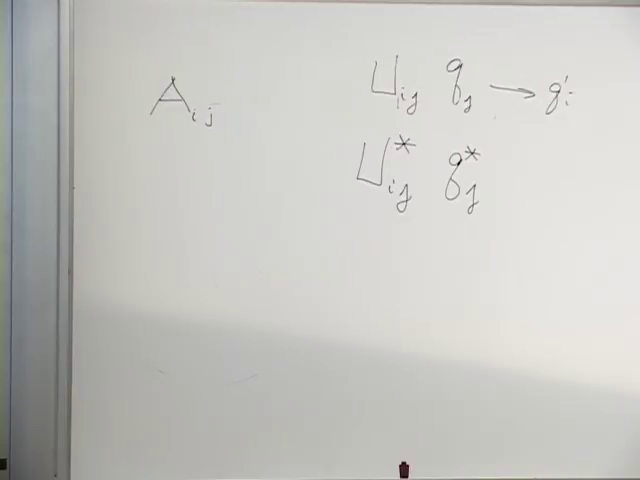
\includegraphics[width=0.62\textwidth]{lecture_05_figure_03.png}
\caption{La transformación fundamental y la transformación conjugada compleja del antitriplete.}
\lectureframe{00:18:47}
\end{figure}

\begin{classroomqa}\audiencequestion{¿Cuántas matrices \(U\) hay--, ¿siete, ocho o nueve?
\lecturetimestamp{00:19:37}}\lecturerresponse{Hay infinitos elementos del grupo \(U\). Lo que se cuenta es el número finito de generadores independientes: ocho para \(SU(3)\). Una matriz general \(3\times3\) tiene nueve posiciones matriciales, pero la unitariedad especial deja ocho direcciones continuas.}\end{classroomqa}

El campo de gluones puede escribirse como una matriz sin traza \(A_{ij}\). Un índice se transforma como el de un quark y el otro como el de un antiquark, de modo que su estructura de color es la de
\begin{equation}
\boldsymbol 3\otimes\bar{\boldsymbol 3}
=\boldsymbol 1\oplus\boldsymbol 8.
\end{equation}
La QCD conserva el octete sin traza,
\begin{equation}
A_{ii}=\operatorname{tr}A=0,
\end{equation}
y descarta el singlete. Por eso la QCD tiene ocho gluones y no nueve. En general, \(SU(N)\) tiene
\begin{equation}
N^2-1
\end{equation}
generadores y el mismo número de campos de bosones gauge.

El fotón es neutro bajo \(U(1)\) eléctrico: rotar la fase de un electrón no transforma el fotón en otro fotón distinto. Los gluones son diferentes. Un gluón lleva un color y un anticolor, así que se transforma en la representación adjunta. Por ejemplo, una combinación rojo--antiazul no es un singlete de color, aunque contenga un color y un anticolor.

\subsection{Flujo de índices e interacción propia}

La regla de interacción puede entenderse siguiendo los índices. Esquemáticamente, un quark de color \(i\) puede convertirse en un quark de color \(j\) al emitir un gluón que lleva el flujo de color correspondiente:
\begin{equation}
q_i\longrightarrow q_j+A_{ij}.
\label{eq:l5-quark-gluon-vertex}
\end{equation}
La posición exacta de \(i\) y \(j\) depende de la convención para las flechas; lo que permanece invariante es que cada índice que entra en un vértice debe continuar por otra línea. No se pierde ningún índice de color.

Esta regla se aplica en cualquier teoría gauge \(SU(N)\). La materia fundamental tiene un índice, la materia antifundamental tiene un índice conjugado y un bosón gauge tiene uno de cada tipo. Los nombres físicos pueden cambiar, pero la estructura de índices permanece.

Como el propio gluón lleva color, puede emitir otro gluón. Un gluón \(A_{ij}\) puede desdoblarse a través de un índice intermedio \(k\), esquemáticamente:
\begin{equation}
A_{ij}\longrightarrow A_{ik}+A_{kj}.
\label{eq:l5-three-gluon-index}
\end{equation}
Este no es un vértice completo de Yang--Mills, pero muestra el flujo de color. En la electrodinámica ordinaria no ocurre nada análogo con los fotones. Por tanto, los gluones ejercen fuerzas sobre otros gluones y la dinámica de un campo no abeliano es mucho más complicada que la teoría lineal de Maxwell.

Una consecuencia cualitativa es el confinamiento. Las líneas de flujo de color no pueden terminar, y su interacción propia las reúne en un tubo que une un quark con un antiquark. El tubo transporta una energía aproximadamente constante por unidad de longitud:
\begin{equation}
V(R)\simeq \sigma R.
\end{equation}
Por tanto, al separar más los extremos se almacena más energía, en vez de liberar color aislado. Esta es la imagen de la «cola pegajosa»: el propio campo impide que los constituyentes coloreados escapen como partículas libres.

\section{Acoplamientos y significado de fuerte o débil}

\subsection{La carga como amplitud de emisión}

Una teoría gauge también necesita una constante de acoplamiento. En la QED, la carga del electrón \(e\) es el coeficiente asociado a un vértice electrón--fotón. Es una amplitud, y las probabilidades son los cuadrados de las amplitudes. Operativamente, imaginemos que detenemos bruscamente un electrón rápido en un tubo de rayos catódicos. La probabilidad de que emita un fotón es proporcional a \(e^2\), con los factores convencionales incluidos en la constante de estructura fina:
\begin{equation}
\alpha=\frac{e^2}{4\pi\hbar c}
\simeq \frac{1}{137}.
\label{eq:l5-alpha}
\end{equation}
En unidades naturales \(\hbar=c=1\), el acoplamiento es adimensional. Una escala del uno por ciento para una emisión elemental hace que el electromagnetismo sea débil en sentido perturbativo: al detenerse, la mayoría de los electrones no emite un chorro de fotones de alta energía.

\subsection{Las unidades naturales relacionan energía, tiempo y distancia}

Tomemos
\begin{equation}
c=1,
\qquad
\hbar=1.
\end{equation}
Entonces el tiempo y la distancia tienen las mismas unidades, mientras que la energía tiene unidades inversas:
\begin{equation}
E=\hbar\omega\longrightarrow E=\omega\sim\frac1t,
\qquad
x\sim t\sim\frac1E.
\end{equation}
Las energías altas sondean distancias y tiempos cortos.

Para orientarnos,
\begin{equation}
1\ {\rm eV}^{-1}
=\frac{\hbar c}{1\ {\rm eV}}
\simeq 1.97\times10^{-7}\ {\rm m}.
\end{equation}
Por tanto, una longitud atómica del orden de \(10^{-10}\ {\rm m}\) corresponde aproximadamente al inverso de un kiloelectronvoltio. Son conversiones de orden de magnitud, no medidas espectroscópicas de precisión.

\subsection{La jerarquía dentro de un átomo}

Para un átomo típico, tomemos
\begin{equation}
R_{\rm atom}\sim10^{-10}\ {\rm m}.
\end{equation}
La luz recorre esta distancia en
\begin{equation}
t_{\rm transit}^{\rm atom}\sim10^{-18}\ {\rm s}.
\end{equation}
Sin embargo, en un átomo ligero el electrón se mueve a una fracción pequeña de la velocidad de la luz. En el modelo de Bohr \(v/c\sim\alpha\), así que el tiempo orbital típico es mayor:
\begin{equation}
t_{\rm orbit}^{\rm atom}\sim10^{-16}\ {\rm s}.
\end{equation}

Un átomo excitado tarda todavía más en emitir radiación:
\begin{equation}
t_{\rm decay}^{\rm atom}\sim10^{-9}\ {\rm s}
\end{equation}
como estimación aproximada a escala de la clase. En el cuadro físico hay dos factores de supresión. La fuerza electromagnética produce solo una aceleración moderada, y un electrón acelerado tiene además una probabilidad de emisión pequeña, controlada por \(\alpha\). Así pues, la pequeña constante de estructura fina genera una jerarquía entre los tiempos de tránsito, orbital y de desintegración radiativa.

\subsection{La ausencia de jerarquía en un hadrón}

Un hadrón es un sistema ligado, similar a un átomo, formado por quarks y gluones, pero su escala es mucho menor:
\begin{equation}
R_{\rm hadron}\sim10^{-15}\ {\rm m},
\qquad
t_{\rm transit}^{\rm hadron}\sim10^{-23}\ {\rm s}.
\end{equation}
Los quarks atraviesan el hadrón prácticamente en la misma escala temporal, y los hadrones excitados que se desintegran por interacción fuerte también viven aproximadamente
\begin{equation}
t_{\rm orbit}^{\rm hadron}
\sim t_{\rm decay}^{\rm hadron}
\sim10^{-23}\ {\rm s}.
\end{equation}
Un hadrón golpeado puede vibrar y emitir un pión casi tan rápido como permite la causalidad. No hay una separación de siete o nueve órdenes de magnitud como la que existe dentro de un átomo.

\begin{classroomqa}\audiencequestion{¿Implica la relatividad especial que un hadrón no puede desintegrarse sustancialmente más rápido que su tiempo de cruce de la luz?
\lecturetimestamp{00:47:15}}\lecturerresponse{Es una manera razonable de expresar el límite de orden de magnitud. Las desintegraciones fuertes ocurren tan rápido como permite el tamaño del sistema; ningún acoplamiento pequeño ni otra supresión grande las ralentiza.}\end{classroomqa}

Por tanto, el acoplamiento fuerte correspondiente es mucho mayor que \(\alpha\). Para una escala hadrónica ilustrativa, la clase cita
\begin{equation}
\alpha_{\rm QCD}\sim0.2,
\end{equation}
un valor mucho más cercano a la unidad que \(1/137\). Este es el origen dinámico del antiguo nombre de \emph{interacciones fuertes}.
\editorialnote{El acoplamiento de la QCD varía con la energía, así que \(\alpha_s\) no es un número fijo. El valor citado es ilustrativo y depende de la escala, tal como se pretende en la clase.}

\begin{classroomqa}\audiencequestion{¿Se llama simplemente constante de la fuerza fuerte a su análogo fuerte?
\lecturetimestamp{00:48:17}}\lecturerresponse{Convencionalmente se llama \(\alpha_{\rm QCD}\) o, más a menudo, \(\alpha_s\). El acoplamiento electromagnético suele llamarse simplemente \(\alpha\), aunque puede usarse \(\alpha_{\rm QED}\) cuando ambos aparecen en la misma discusión.}\end{classroomqa}

\begin{classroomqa}\audiencequestion{¿En un artículo se distinguiría entre un acoplamiento electromagnético desnudo y el valor medido, apantallado?
\lecturetimestamp{00:48:38}}\lecturerresponse{Sí. Se habla de acoplamiento desnudo y de acoplamiento renormalizado. La polarización del vacío hace que el acoplamiento efectivo dependa de la escala a la que se mide.}\end{classroomqa}

\section{El enigma de la desintegración débil}

Las interacciones débiles recibieron ese nombre por sus tiempos de desintegración muy largos. Suelen ser más lentas que las desintegraciones fuertes e incluso pueden ser más lentas que la radiación atómica. El ejemplo más antiguo es la desintegración beta nuclear.

\subsection{Desintegración beta del neutrón}

Un neutrón libre se desintegra mediante
\begin{equation}
n\longrightarrow p+e^-+\bar\nu_e.
\label{eq:l5-neutron-decay-intro}
\end{equation}
La clase emplea una vida media de unos doce minutos, absurdamente larga en comparación con \(10^{-23}\ {\rm s}\). Para el argumento no importan los valores modernos de precisión.

Parte de la lentitud es cinemática. Aproximadamente,
\begin{equation}
\begin{aligned}
m_n&\simeq940\ {\rm MeV},
&
m_p&\simeq939\ {\rm MeV},
\\
m_e&\simeq0.5\ {\rm MeV}.
\end{aligned}
\end{equation}
Solo una fracción diminuta de la energía en reposo del neutrón queda disponible como energía cinética. Si el neutrón tuviera menos masa que la suma de las masas en reposo finales, la desintegración sería imposible. Si su masa apenas superara el umbral, el espacio de fases disponible sería diminuto y la desintegración sería lenta. Pero el espacio de fases por sí solo no puede explicar una vida media de minutos.

\subsection{El pión cargado descarta la explicación del umbral}

Consideremos también
\begin{equation}
\pi^-\longrightarrow e^-+\bar\nu_e
\end{equation}
y el proceso conjugado en carga. El pión tiene energía más que suficiente por encima del umbral del canal electrónico; aun así, su vida media débil es del orden de los nanosegundos, no del orden de \(10^{-23}\) segundos, como en los procesos hadrónicos. Pronto cobrará importancia un canal análogo con un muón. Por tanto, el enigma es propio de la interacción débil y no se debe simplemente a la casi degeneración de las masas del neutrón.

\editorialnote{La vida media del pión cargado es de unos \(26\ {\rm ns}\) y el canal dominante es \(\pi^-\to\mu^-\bar\nu_\mu\). El canal electrónico está suprimido por helicidad. La clase comienza con el canal electrónico porque su recuento de partículas es el más sencillo y luego vuelve al canal dominante con muones.}

El término desintegración beta proviene históricamente de que se llamaba rayos beta a los electrones emitidos. Los ejemplos del pión y del neutrón implican la misma interacción de corriente cargada, aunque su cinemática difiere considerablemente.

\section{Tabla de quarks y leptones}

\subsection{El color actúa en vertical}

Distribuyamos los seis sabores de quarks en tres columnas de pares,
\begin{equation}
(u,d),\qquad(c,s),\qquad(t,b),
\end{equation}
y coloquemos una copia roja, verde y azul de cada quark en filas separadas. El color \(SU(3)\) actúa en vertical: transforma entre sí las versiones roja, verde y azul de un quark up y realiza simultáneamente la misma rotación de color en los quarks down, charm, strange, top y bottom. No transforma un quark up en uno down.

\subsection{El isoespín débil actúa en horizontal}

La simetría débil actúa en la otra dirección. Mezcla cada par contiguo
\begin{equation}
Q_1=\begin{pmatrix}u\\d\end{pmatrix},
\qquad
Q_2=\begin{pmatrix}c\\s\end{pmatrix},
\qquad
Q_3=\begin{pmatrix}t\\b\end{pmatrix}.
\label{eq:l5-quark-doublets}
\end{equation}
Los quarks de tipo up tienen carga \(+2/3\) y los de tipo down, carga \(-1/3\), así que la carga cambia en una unidad a través de cada par.
\editorialnote{En la fuente se dice por un instante que un quark down tiene carga \(-2/3\). La resta que aparece alrededor y todos los procesos posteriores requieren el valor estándar \(-1/3\), que es el que se usa aquí.}

Como la simetría actúa sobre dobletes, el grupo natural es \(SU(2)\). Actúa sobre cada copia de color de cada doblete de quarks sin cambiar el color.

También hay una cuarta fila de partículas que no llevan color y, por tanto, no interactúan con los gluones: los leptones. Forman otros tres dobletes,
\begin{equation}
L_e=\begin{pmatrix}\nu_e\\e^-\end{pmatrix},
\qquad
L_\mu=\begin{pmatrix}\nu_\mu\\\mu^-\end{pmatrix},
\qquad
L_\tau=\begin{pmatrix}\nu_\tau\\\tau^-\end{pmatrix}.
\label{eq:l5-lepton-doublets}
\end{equation}
Los neutrinos son eléctricamente neutros; el electrón, el muón y el tau tienen carga \(-1\). De nuevo, los dos miembros difieren en una unidad de carga eléctrica. El electrón, el muón y el tau tienen los mismos números cuánticos gauge, pero masas diferentes, igual que las tres generaciones de quarks de tipo up o de tipo down repiten el mismo patrón de cargas.

\begin{figure}[htbp]
\centering
\includegraphics[width=0.82\textwidth]{lecture_05_figure_05.png}
\caption{La tabla de la pizarra: el color actúa entre las filas roja, azul y verde, mientras que \(SU(2)\) débil conecta las columnas de sabores emparejados y la fila de leptones.}
\lectureframe{01:03:35}
\end{figure}

Llamar a los leptones un cuarto color es solo una analogía en esta etapa. Ocupan una cuarta fila en la tabla de dobletes débiles, pero la QCD ordinaria \(SU(3)\) no transforma quarks en leptones.

\section{Construcción de los bosones débiles cargados}

\subsection{Números cuánticos de los bosones cargados}

Los bosones gauge llevan las propiedades de transformación necesarias para pasar de un miembro del doblete al otro. Empecemos con el par de leptones \(e^-\bar\nu_e\). Tiene carga eléctrica \(-1\), así que el bosón gauge cargado correspondiente se llama \(W^-\):
\begin{equation}
W^-\sim e^-\bar\nu_e.
\end{equation}
Se obtienen los mismos números cuánticos a partir de un quark down y un antiquark up:
\begin{equation}
W^-\sim d\bar u.
\end{equation}
El símbolo \(\sim\) significa «tiene los mismos números cuánticos gauge pertinentes que». No significa que \(W\) sea literalmente un estado ligado de estas partículas. La antipartícula tiene las combinaciones conjugadas:
\begin{equation}
W^+\sim e^+\nu_e\sim\bar d u.
\end{equation}

Los vértices débiles cargados incluyen
\begin{align}
e^-&\longrightarrow\nu_e+W^-,
&
\mu^-&\longrightarrow\nu_\mu+W^-,
\label{eq:l5-lepton-w}\\
d&\longrightarrow u+W^-,
&
s&\longrightarrow c+W^-,
\label{eq:l5-quark-w}
\end{align}
con transiciones análogas para la tercera generación cuando la cinemática lo permite. El bosón gauge realiza dinámicamente la misma mezcla horizontal que la simetría lleva a cabo en el doblete.

\begin{classroomqa}\audiencequestion{La conservación de la carga exige que el bosón emitido tenga carga \(-1\), pero ¿por qué las transiciones del electrón, del quark down y del quark strange implican todas la misma partícula?
\lecturetimestamp{01:12:56}}\lecturerresponse{Es un hecho empírico codificado por la simetría débil común. La naturaleza podría haber asignado de manera coherente un bosón de tipo \(W\) distinto a cada familia o por separado a los quarks y los leptones. En cambio, un solo \(SU(2)\) actúa simultáneamente sobre todos los dobletes, y los mismos bosones gauge cargados median todas estas transiciones.}\end{classroomqa}

\subsection{Lectura e inversión de un vértice}

Un solo vértice representa toda una familia de procesos. Invertir una línea entrante para convertirla en saliente transforma una partícula en su antipartícula, e invertir una línea \(W^-\) da una \(W^+\). Por tanto, un vértice puede interpretarse como emisión, absorción, desintegración, aniquilación o la reacción inversa, siempre que se sigan de forma coherente la carga, el momento y todos los números cuánticos pertinentes.

\begin{classroomqa}\audiencequestion{¿Se pueden invertir las flechas y las líneas de estos vértices débiles?
\lecturetimestamp{01:14:51}}\lecturerresponse{Sí. Una línea puede cruzarse del estado final al inicial, o viceversa, pero entonces una partícula se convierte en su antipartícula. En consecuencia, el mismo vértice local describe muchas reacciones con orientaciones distintas.}\end{classroomqa}

\begin{classroomqa}\audiencequestion{Si se dibuja un \(W^-\) con líneas de strange y charm, ¿significa que el bosón es literalmente un quark strange ligado a un antiquark charm?
\lecturetimestamp{01:15:43}}\lecturerresponse{No. El recuento de líneas solo indica que el \(W^-\) lleva el cambio de números cuánticos entre esas columnas. Si el diagrama se interpreta como una desintegración, un \(W^-\) suficientemente energético puede producir un quark strange y un antiquark charm; no está compuesto por ellos.}\end{classroomqa}

\begin{classroomqa}\audiencequestion{¿Pueden un electrón y un antineutrino formar un \(W\) que luego produzca un par de quarks?
\lecturetimestamp{01:17:22}}\lecturerresponse{Exactamente. Si hay suficiente energía en el centro de masas, los leptones iniciales pueden formar el estado intermedio de corriente cargada, que puede manifestarse a través de un canal de quarks permitido. Son los mismos dos vértices que aparecen en una desintegración, pero leídos con otra orientación.}\end{classroomqa}

\subsection{El tercer bosón que falta}

El grupo \(SU(2)\) tiene tres generadores y, por tanto, tres campos gauge. Hasta ahora solo hemos mostrado \(W^+\) y \(W^-\). Debe haber un tercer campo eléctricamente neutro asociado a combinaciones diagonales, como las correspondientes a los números cuánticos electrón--positrón y neutrino--antineutrino. Se deja deliberadamente en segundo plano. Su relación con el bosón \(Z\) físico y el fotón requiere la mezcla electrodébil, que veremos más adelante.

\begin{classroomqa}\audiencequestion{¿Se sospechó de las fuerzas débil y fuerte en épocas históricas distintas?
\lecturetimestamp{01:24:11}}\lecturerresponse{Sus raíces experimentales aparecieron juntas en los primeros estudios de la radiactividad. La desintegración alfa reveló la física nuclear y de la interacción fuerte; la desintegración beta, la interacción débil; y la desintegración gamma emitía fotones electromagnéticos. En la época de Becquerel ya estaban presentes las tres pistas, mucho antes de que existieran sus teorías de campos modernas.}\end{classroomqa}

\section{Ejemplos resueltos de desintegraciones de corriente cargada}

\subsection{Desintegración del pión}

El pión con carga negativa tiene el contenido de quarks de valencia
\begin{equation}
\pi^-=d\bar u.
\end{equation}
Esos números cuánticos pueden aniquilarse y producir un \(W^-\), que a su vez puede producir un leptón cargado y el antineutrino correspondiente:
\begin{align}
\pi^-&\longrightarrow W^{-*}
\longrightarrow e^-+\bar\nu_e,
\label{eq:l5-pion-electron}\\
\pi^-&\longrightarrow W^{-*}
\longrightarrow \mu^-+\bar\nu_\mu.
\label{eq:l5-pion-muon}
\end{align}
El asterisco indica que el \(W\) intermedio es virtual. El segundo canal es el dominante.

\begin{figure}[htbp]
\centering
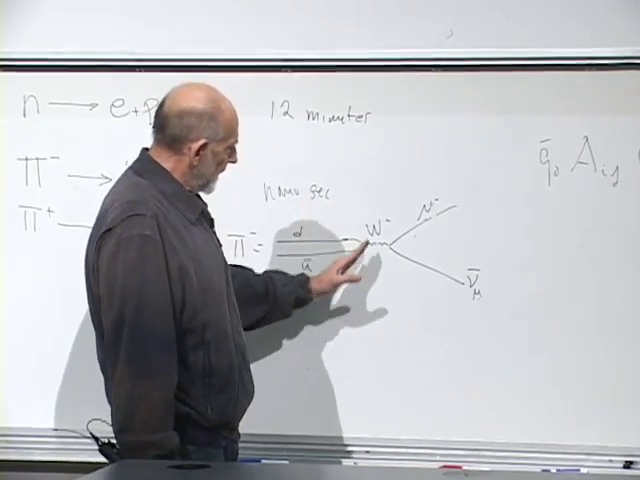
\includegraphics[width=0.72\textwidth]{lecture_05_figure_04.png}
\caption{Un pión \(d\bar u\) se aniquila y produce un \(W^-\) virtual, seguido de un leptón cargado y su antineutrino correspondiente.}
\lectureframe{01:19:38}
\end{figure}

\begin{classroomqa}\audiencequestion{¿Sigue siendo esto realmente un diagrama de Feynman aunque la dirección del tiempo se haya dibujado en horizontal y no en vertical?
\lecturetimestamp{01:20:21}}\lecturerresponse{Sí. La orientación del tiempo en la página es una convención. Una vez declarada una dirección como temporal e interpretadas todas las flechas de manera coherente, el dibujo contiene la misma información sobre la interacción.}\end{classroomqa}

\begin{classroomqa}\audiencequestion{¿Podría leerse el diagrama como una reacción química reversible, en lugar de como una desintegración irreversible en un solo sentido?
\lecturetimestamp{01:21:35}}\lecturerresponse{El proceso inverso está permitido. Un pión producido en el espacio vacío se desintegra porque las partículas salientes se separan y normalmente no vuelven a combinarse. Pero si se hacen colisionar un muón y un antineutrino con la energía y el momento adecuados, existe una amplitud no nula para formar el pión mediante la interacción inversa.}\end{classroomqa}

\subsection{Energía y estado intermedio virtual}

Para un pión en reposo,
\begin{equation}
m_\pi\simeq140\ {\rm MeV},
\qquad
m_\mu\simeq106\ {\rm MeV},
\qquad
m_\nu\approx0
\end{equation}
con la precisión pertinente aquí. La energía restante se convierte en energía cinética de las partículas salientes. La conservación del momento exige
\begin{equation}
\boldsymbol p_\mu+\boldsymbol p_{\bar\nu}=0,
\end{equation}
por lo que las dos partículas salen en direcciones opuestas en el sistema de referencia en reposo del pión.

\begin{classroomqa}\audiencequestion{¿Cómo puede conservarse la energía si el \(W\) intermedio tiene una masa muy superior a la del pión?
\lecturetimestamp{01:25:08}}\lecturerresponse{Solo las partículas iniciales y finales deben estar en su capa de masa. El cuadrimomento se conserva en cada vértice, pero una línea virtual interna no tiene por qué satisfacer \(E^2=\boldsymbol p^2+m_W^2\). Cuanto mayor es su desviación respecto de la capa de masa, más suprime el proceso su propagador.\editorialnote{La clase recurre al lenguaje tradicional de la incertidumbre energía--tiempo y dice que el estado intermedio puede violar brevemente la conservación de la energía. La formulación moderna y precisa es la de la respuesta: se conserva la energía y el momento, mientras que una línea interna virtual no tiene por qué satisfacer la condición de capa de masa de una partícula real.}}
\end{classroomqa}

\subsection{Desintegración del muón}

Un muón puede transformarse primero en su propio neutrino al emitir un \(W^-\) virtual:
\begin{equation}
\mu^-\longrightarrow\nu_\mu+W^{-*}.
\end{equation}
El bosón virtual produce luego un electrón y un antineutrino electrónico:
\begin{equation}
\mu^-\longrightarrow
\nu_\mu+e^-+\bar\nu_e.
\label{eq:l5-muon-decay}
\end{equation}
Este es un proceso puramente leptónico. El muón tiene una masa unas doscientas veces mayor que la del electrón, así que las masas en reposo finales dejan energía cinética suficiente.

\begin{figure}[htbp]
\centering
\includegraphics[width=0.72\textwidth]{lecture_05_figure_06.png}
\caption{Desintegración del muón a través de un bosón débil cargado virtual.}
\lectureframe{01:29:24}
\end{figure}

\begin{classroomqa}
\audiencequestion{¿La partícula neutra emitida junto con el electrón es un
antineutrino?
\lecturetimestamp{01:29:06}}
\lecturerresponse{Sí. El estado final completo contiene un neutrino muónico, un
antineutrino electrónico y el electrón. Mantener las etiquetas de sabor evita
confundir las dos partículas neutras.}
\end{classroomqa}

El electrón no puede invertir este decaimiento en el espacio vacío porque es más ligero que el muón. El tau es más pesado y puede decaer por canales débiles análogos. La estabilidad en este caso se debe en parte a una coincidencia del orden de las masas, no a una diferencia en el vértice subyacente.

\begin{classroomqa}
\audiencequestion{¿Un acelerador lineal aumenta, en la práctica, la masa del
electrón para que las reacciones que de otro modo estarían prohibidas puedan
producirse en sentido contrario?
\lecturetimestamp{01:30:23}}
\lecturerresponse{No cambia la masa invariante en reposo del electrón, pero
le proporciona energía cinética. Una energía suficiente en el centro de masas
puede crear partículas finales más pesadas; por tanto, la idea física propuesta
es correcta si se sustituye la masa por la energía de colisión disponible.}
\end{classroomqa}

\subsection{Decaimiento beta del neutrón a nivel de quarks}

Las composiciones de quarks de valencia del neutrón y el protón son
\begin{equation}
n=udd,
\qquad
p=uud.
\end{equation}
Un quark down del neutrón experimenta la transición de corriente cargada
\begin{equation}
d\longrightarrow u+W^{-*},
\end{equation}
que convierte \(udd\) en \(uud\). Luego, el bosón virtual decae:
\begin{equation}
W^{-*}\longrightarrow e^-+\bar\nu_e.
\end{equation}
La combinación de ambos vértices reproduce
\begin{equation}
n\longrightarrow p+e^-+\bar\nu_e.
\end{equation}

La transición inversa del quark \(u\to d+W^+\) daría lugar a un barión formado por tres quarks down, pero ese estado accesible tiene demasiada masa para que lo produzca un neutrón libre. La vía real de down a up es la que está permitida energéticamente.

\begin{classroomqa}
\audiencequestion{¿Podría decaer un neutrón en un protón, un muón y el
antineutrino correspondiente?
\lecturetimestamp{01:32:38}}
\lecturerresponse{No, si el neutrón libre está en reposo: la diferencia de masas entre el neutrón--y el protón es mucho menor que la masa del muón. Con suficiente energía adicional de colisión o de excitación, el mismo vértice débil puede participar en un canal que produzca un muón. La prohibición es cinemática; no se debe a la ausencia de una interacción.}
\end{classroomqa}

\section{La supresión aún sin explicar}

Los vértices débiles cargados explican qué procesos pueden ocurrir, pero todavía no por qué son tan lentos. Una respuesta tentadora sería que el acoplamiento débil es extraordinariamente pequeño. Esa respuesta es incorrecta: el acoplamiento gauge débil adimensional es de un orden de magnitud similar al electromagnético. La supresión debe tener otro origen.

El ingrediente que falta ya se aprecia en el propagador virtual: el \(W\) tiene una masa muy grande. A energías muy inferiores a \(m_W\), las amplitudes de corriente cargada se suprimen aproximadamente mediante potencias de \(1/m_W^2\). Esta conexión se desarrollará después de explicar cómo el mecanismo de Higgs y la ruptura de la simetría electrodébil dan masa a los bosones gauge.
\editorialnote{La clase deja planteada esta cuestión para la próxima sesión. La explicación basada en el bosón pesado \(W\) se incluye aquí como anticipo, no como afirmación de que su derivación haya tenido lugar en esta clase.}

\begin{classroomqa}
\audiencequestion{Cuando decimos que la teoría tiene esta simetría, ¿queremos
decir que su lagrangiano es invariante bajo las operaciones correspondientes?
\lecturetimestamp{01:34:14}}
\lecturerresponse{Exactamente. Decir que la teoría tiene la simetría es una
forma abreviada de afirmar que el lagrangiano, o equivalentemente la acción, es
invariante bajo esas transformaciones. La escritura del lagrangiano completo se
pospone; no se sustituye por una definición distinta.}
\end{classroomqa}

La exposición llega así a su conclusión: la teoría de Maxwell proporciona el prototipo; la cromodinámica cuántica muestra cómo los bosones gauge no abelianos transportan e intercambian carga; las constantes de acoplamiento explican el contraste entre las escalas de tiempo atómicas y hadrónicas; y \(SU(2)\) organiza los quarks y los leptones en dobletes conectados por \(W^\pm\). Queda por entender por qué, en la práctica, estos procesos mediados por bosones gauge son débiles, aunque el acoplamiento subyacente no sea excepcionalmente pequeño.
